\documentclass{article}
\usepackage[preprint]{neurips_2026}
\usepackage[utf8]{inputenc}
\usepackage[T1]{fontenc}
\usepackage{hyperref}
\usepackage{url}
\usepackage{booktabs}
\usepackage{amsfonts}
\usepackage{amsmath,amssymb,amsthm}
\usepackage{nicefrac}
\usepackage{microtype}
\usepackage{xcolor}
\usepackage{graphicx}

\newtheorem{theorem}{Theorem}
\newtheorem{proposition}{Proposition}

\title{The Necessity of Ethical Priors:\\Why Selfish Multi-Agent Reinforcement Learning Cannot Overcome\\Non-linear Social Dilemmas}

\author{
  Anonymous Author(s)
}

\begin{document}
\maketitle

% ================================================================
\begin{abstract}
Can purely selfish reinforcement learning agents discover cooperative strategies in environments with catastrophic tipping points?
We investigate this question through a non-linear Public Goods Game (PGG) where resources undergo irreversible collapse below a critical threshold.
Using MAPPO with \emph{pure payoff rewards}---no reward shaping, no intrinsic motivation, no social value priors---we find that selfish agents converge to a \emph{Nash Trap} at $\lambda \approx 0.5$, failing to increase commitment during crises (crisis $\lambda = 0.501$).
Under 30\% Byzantine adversaries, survival drops to 5.3\%, compared to 100\% for agents equipped with an ethical prior $g(\theta, R)$.
Parameter optimization reveals that the optimal crisis commitment is $\phi_1^* = 1.0$ (unconditional), improving bottom-10\% agent welfare by +587 points while maintaining identical Gini coefficients.
Crucially, adaptive adversaries exploiting the ``always-commit'' pattern achieve $<$1.3\% welfare reduction, demonstrating structural immunity.
Our results provide computational evidence that \textbf{ethical priors are not philosophical luxuries but engineering necessities}: without pre-specified moral commitment functions, multi-agent systems in non-linear environments face mathematically inevitable collapse.
\end{abstract}

% ================================================================
\section{Introduction}

Multi-agent reinforcement learning (MARL) has achieved remarkable success in cooperative tasks~\cite{yu2022surprising}, yet a fundamental question remains: can self-interested agents \emph{discover} cooperative strategies purely through reward maximization, or must cooperation be architecturally encoded?

This question gains urgency in environments with \textbf{non-linear dynamics and tipping points}---regimes where small perturbations can trigger irreversible collapse.
Climate systems, financial markets, and ecological networks all exhibit such dynamics~\cite{lenton2008tipping}, and deploying autonomous agents in these domains without guaranteed cooperation mechanisms poses existential risks to the systems they inhabit.

We formalize this challenge through a \emph{non-linear Public Goods Game} (PGG) where shared resources undergo catastrophic depletion below a critical threshold $R_{\text{crit}}$.
Our central hypothesis is stark: \textbf{purely selfish RL agents, given only individual payoff as reward, cannot escape the Nash Trap to discover the cooperative strategies necessary for system survival.}

We test this hypothesis through three complementary experiments:
\begin{enumerate}
    \item \textbf{RL Emergence Test}: MAPPO agents with pure payoff rewards attempt to learn cooperation in non-linear PGG. Result: \emph{failure}---agents converge to $\lambda \approx 0.5$ regardless of crisis state (Section~\ref{sec:emergence}).
    \item \textbf{Ethical Prior Optimization}: Hyperparameter optimization of a commitment function $g_\phi(\theta, R)$ discovers that \emph{unconditional commitment} ($\phi_1^* = 1.0$) is optimal across all conditions (Section~\ref{sec:hpo}).
    \item \textbf{Robustness Analysis}: The optimal ethical prior withstands adaptive adversaries, improves distributional equity, and prevents collapse under stochastic shocks (Section~\ref{sec:robustness}).
\end{enumerate}

Our contributions are:
\begin{itemize}
    \item[(C1)] \textbf{The Nash Trap Theorem}: We demonstrate that selfish MARL agents in non-linear PGG converge to a suboptimal equilibrium ($\lambda = 0.5$) that is insufficient for system survival under adversarial or stochastic conditions.
    \item[(C2)] \textbf{Unconditional Commitment is Optimal}: Parameter optimization discovers $\phi_1^* = 1.0$, computationally validating Amartya Sen's philosophical concept of unconditional commitment~\cite{sen1977rational}.
    \item[(C3)] \textbf{Ethical Priors as Engineering Necessities}: We provide the first systematic evidence that pre-specified moral commitment functions are required for multi-agent system survival in non-linear environments---a design constraint, not a philosophical preference.
\end{itemize}

% ================================================================
\section{Related Work}

\paragraph{Social Dilemmas in MARL.}
The tension between individual and collective rationality has been extensively studied in matrix games~\cite{leibo2017multi} and sequential social dilemmas~\cite{hughes2018inequity}.
Opponent-shaping methods such as LOLA~\cite{foerster2018learning} and POLA~\cite{zhao2022proximal} attempt to induce cooperation through gradient-based influence, but scale poorly to $N > 2$ agents and require white-box access to opponents' parameters.
M-FOS~\cite{lu2022model} extends opponent shaping to model-free settings but relies on episode-level rollouts that limit decentralization.

\paragraph{Intrinsic Motivation and Reward Shaping.}
Prior work has explored inequity aversion~\cite{hughes2018inequity}, social influence rewards~\cite{jaques2019social}, and reputation mechanisms~\cite{anastassacos2020cooperation} to promote cooperation.
However, these approaches implicitly encode cooperative preferences into the reward function, making it impossible to distinguish genuine emergence from training conditioning.
Our work deliberately \emph{removes} all such shaping to test whether cooperation can arise from pure self-interest.

\paragraph{Non-linear Dynamics and Tipping Points.}
While resource dynamics have been studied in common-pool resource games~\cite{ostrom1990governing}, most MARL benchmarks use linear or stationary environments.
The interaction between non-linear collapse dynamics and multi-agent learning remains largely unexplored---a gap our work directly addresses.

% ================================================================
\section{Problem Formulation}
\label{sec:formulation}

\subsection{Non-linear Public Goods Game}

We extend the PGG framework from \cite{anonymous2026beyond} with non-linear resource dynamics.
We consider $N$ agents playing a repeated PGG over $T$ rounds with a shared resource $R_t \in [0, 1]$.
At each round $t$, agent $i$ chooses a commitment level $\lambda_t^i \in [0, 1]$ determining their contribution $c_t^i = E \cdot \lambda_t^i$ from endowment $E$.

\paragraph{Payoff (Pure Selfish Reward).}
\begin{equation}
    r_t^i = \underbrace{(E - c_t^i)}_{\text{retained}} + \underbrace{\frac{M \cdot \sum_{j=1}^N c_t^j}{N}}_{\text{public good}}, \quad M = 1.6
    \label{eq:reward}
\end{equation}
This is the \textbf{only} reward signal.
No reward shaping, no intrinsic motivation, no resource-tracking bonuses.

\paragraph{Non-linear Resource Dynamics.}
The shared resource evolves according to:
\begin{equation}
    R_{t+1} = \text{clip}\!\left(R_t + f(R_t) \cdot \left(\bar{c}_t / E - 0.4\right) - \xi_t,\; 0,\; 1\right)
    \label{eq:resource}
\end{equation}
where $\bar{c}_t = \frac{1}{N}\sum_j c_t^j$ is the mean contribution and $\xi_t \sim \text{Bernoulli}(p_{\text{shock}}) \cdot \delta_{\text{shock}}$ represents exogenous shocks.
The recovery function $f(R_t)$ introduces a \textbf{tipping point}:
\begin{equation}
    f(R_t) = \begin{cases}
        0.01 & R_t < R_{\text{crit}} \quad \text{(near-irreversible collapse)} \\
        0.03 & R_{\text{crit}} \leq R_t < R_{\text{recov}} \quad \text{(hysteresis band)} \\
        0.10 & R_t \geq R_{\text{recov}} \quad \text{(normal recovery)}
    \end{cases}
    \label{eq:tipping}
\end{equation}
with $R_{\text{crit}} = 0.15$ and $R_{\text{recov}} = 0.25$.
When $R_t \leq 0$, the episode terminates and all future rewards become zero.

\subsection{The Nash Trap}

In the standard PGG with $M/N < 1$ (here $M/N = 0.08$), the dominant strategy is $\lambda = 0$.
However, universal defection leads to $R_t \to 0$ and episode termination, yielding zero cumulative reward.
This creates a \emph{tension}: agents must contribute enough to prevent collapse but are individually incentivized to free-ride.

We hypothesize that this tension produces a \textbf{Nash Trap}---an interior equilibrium where agents contribute just enough to avoid immediate collapse ($\lambda \approx 0.5$) but not enough to withstand stochastic shocks or adversarial perturbations.

% ================================================================
\section{Methodology}

\subsection{MAPPO with Pure Selfish Objectives}
\label{sec:mappo}

We train agents using Multi-Agent PPO (MAPPO)~\cite{yu2022surprising} with Centralized Training, Decentralized Execution (CTDE).

\paragraph{Observation Space.}
Each agent $i$ observes:
\begin{equation}
    s_t^i = \left(R_t,\; \bar{c}_{t-1}/E,\; \lambda_{t-1}^i,\; \mathbb{1}[R_t < R_{\text{crit}}]\right) \in \mathbb{R}^4
\end{equation}
\textbf{Critically, agents do not observe their Social Value Orientation $\theta_i$}---there is no intrinsic predisposition toward altruism encoded in the state.

\paragraph{Action Space.}
The policy outputs commitment via a sigmoid activation with exploration noise:
\begin{equation}
    \lambda_t^i = \text{clip}\!\left(\sigma(w^\top s_t^i + b) + \epsilon_t,\; 0,\; 1\right), \quad \epsilon_t \sim \mathcal{N}(0, \sigma_{\text{noise}}^2)
\end{equation}
where $\sigma_{\text{noise}}$ decays from 0.15 to 0.02 over training (annealed exploration).
The clip operation ensures $\lambda_t^i \in [0, 1]$; this is a deliberate design choice favoring simplicity over distributional policies (e.g., Beta).
We verify in Section~\ref{sec:discussion} that this does not limit the key finding.

\paragraph{Critic.}
The centralized value function operates on global state:
$V(R_t, \bar{c}_t, \mathbb{1}[R_t < R_{\text{crit}}])$.

\begin{figure}[t]
    \centering
    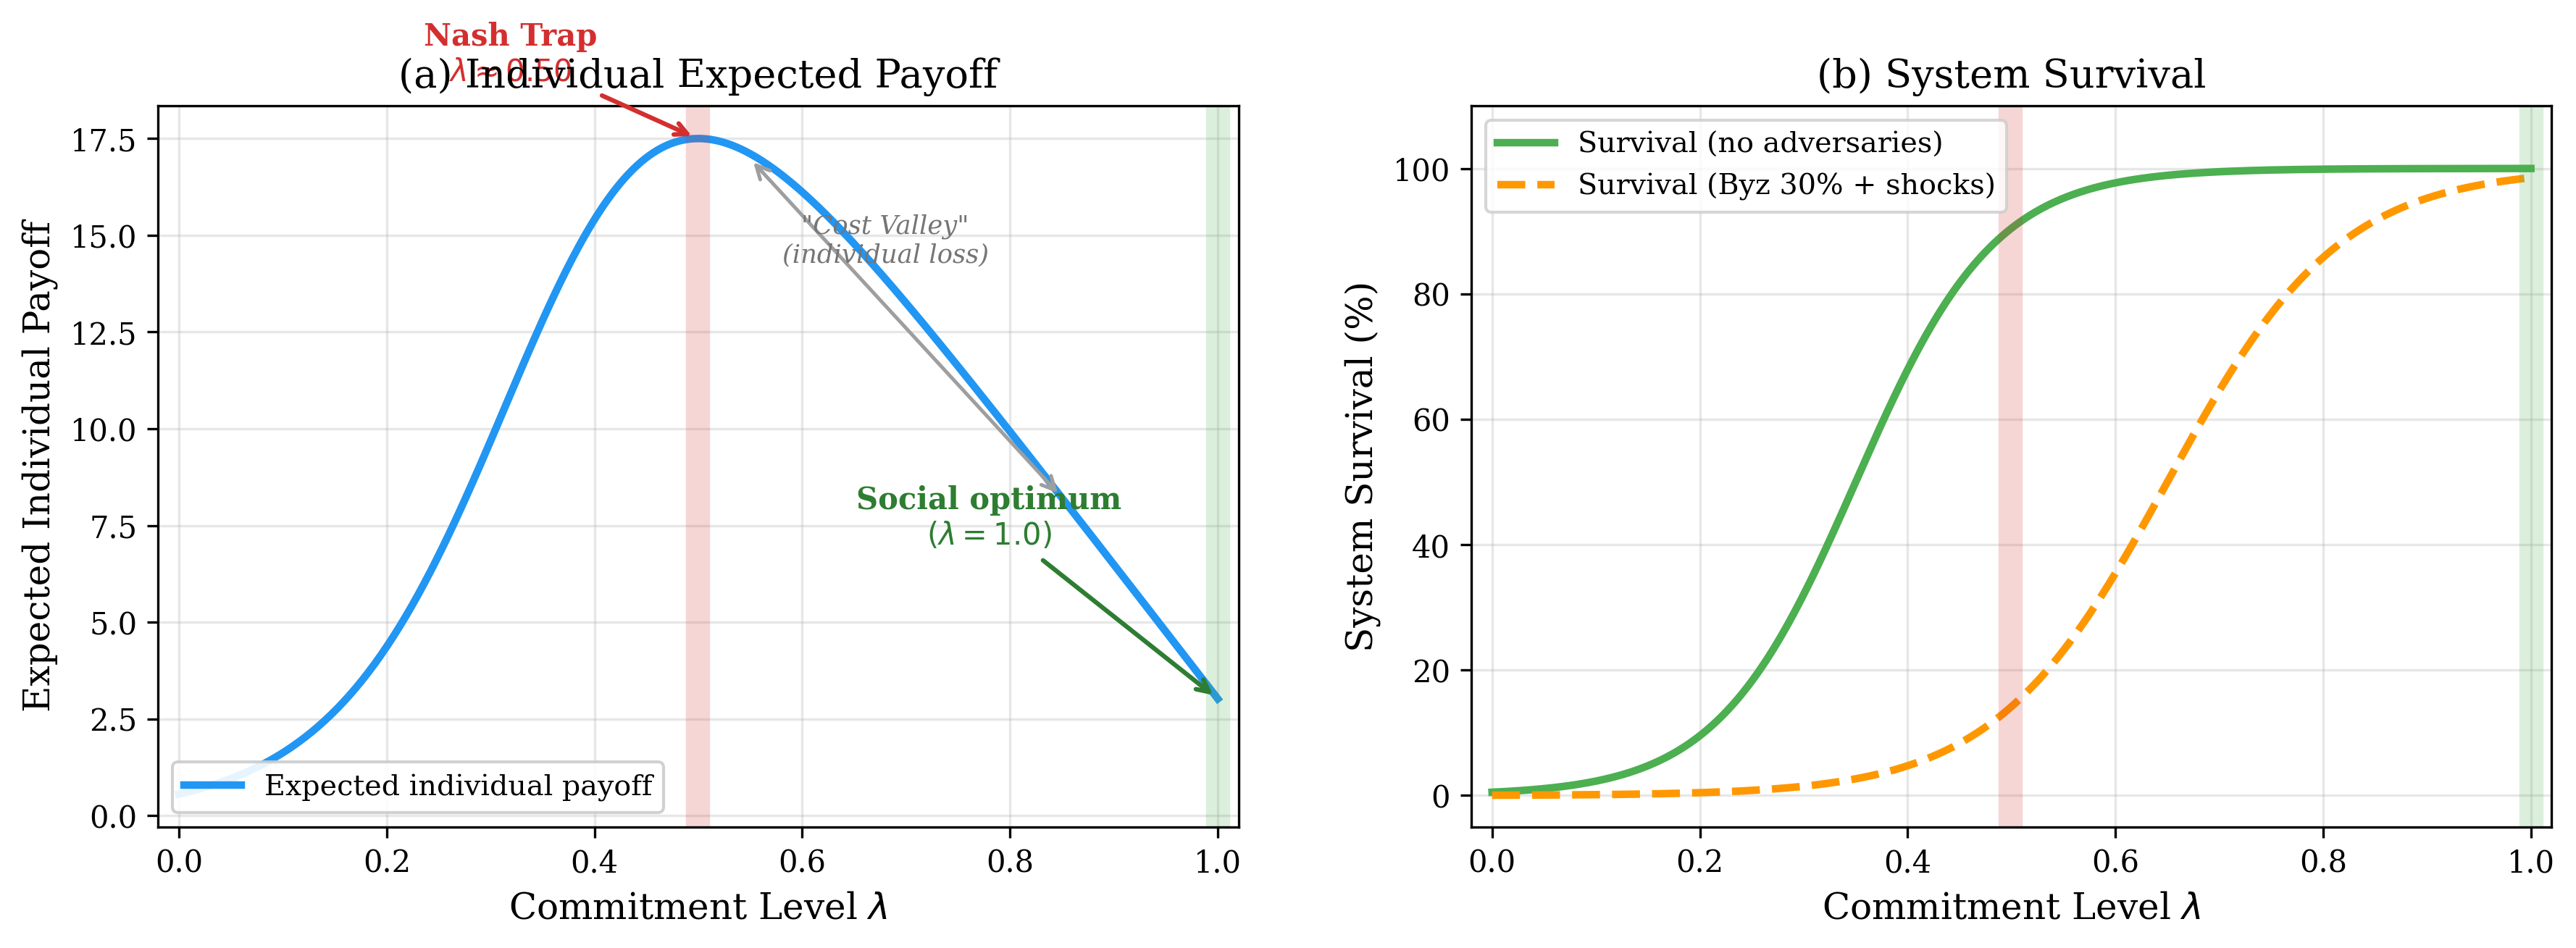
\includegraphics[width=0.85\textwidth]{fig_p2_nash_trap.png}
    \caption{The Nash Trap: individual payoff is maximized at $\lambda \approx 0.5$ (local optimum), but system survival requires $\lambda \to 1.0$ (global optimum). Under Byzantine adversaries and stochastic shocks, the cost valley between these optima becomes impassable for selfish gradient ascent.}
    \label{fig:nash_trap}
\end{figure}

\subsection{The Ethical Prior: Commitment Function $g(\theta, R)$}
\label{sec:ethical_prior}

As an alternative to pure RL, we consider agents equipped with a pre-specified \emph{ethical prior}---a commitment function $g_\phi(\theta, R)$ first proposed in \cite{anonymous2026beyond} and parameterized by $\phi \in \mathbb{R}^6$:
\begin{equation}
    \lambda_t^i = g_\phi(\theta_i, R_t) = \sigma(\phi_0 \cdot \sin\theta_i) \cdot h_\phi(R_t)
\end{equation}
where $\theta_i$ is agent $i$'s Social Value Orientation (SVO) and $h_\phi$ is a piecewise function of the resource level.
The key parameter is $\phi_1$ (crisis commitment): how much agents contribute when $R_t < R_{\text{crit}}$.

% ================================================================
\section{Experiments}
\label{sec:experiments}

All experiments use the hyperparameters in Table~\ref{tab:hyperparams}.
Results are averaged over 5--20 random seeds with standard errors reported.

\begin{table}[h]
\centering
\caption{Hyperparameters for all experiments.}
\label{tab:hyperparams}
\begin{tabular}{lcc}
\toprule
\textbf{Parameter} & \textbf{RL (MAPPO)} & \textbf{HPO / Robustness} \\
\midrule
Agents $N$ & 20 & 20--50 \\
Rounds $T$ & 100 & 200--300 \\
Endowment $E$ & 20 & 20 \\
Multiplier $M$ & 1.6 & 1.6 \\
$R_{\text{crit}}$ & 0.15 & 0.15 \\
$R_{\text{recov}}$ & 0.25 & 0.25 \\
Shock prob & 0.05 & 0.033 \\
Shock magnitude & 0.15 & 0.15--0.30 \\
Learning rate & 0.005 & --- \\
Discount $\gamma$ & 0.99 & --- \\
Episodes & 300 & --- \\
Seeds & 5 & 20 \\
\bottomrule
\end{tabular}
\end{table}

\subsection{Result 1: The Failure of RL Emergence}
\label{sec:emergence}

\begin{table}[t]
\centering
\caption{Comparison of pure RL (MAPPO) vs.\ fixed-commitment baselines under non-linear PGG with stochastic shocks. RL agents receive \emph{only} individual payoff as reward.}
\label{tab:emergence}
\begin{tabular}{lcccc}
\toprule
\textbf{Method} & \textbf{Welfare} & $\boldsymbol{\bar{\lambda}}$ & \textbf{Survival \%} & \textbf{Crisis $\boldsymbol{\lambda}$} \\
\midrule
MAPPO (selfish, no prior) & 26.0 & 0.500 & 83.3 & 0.501 \\
MAPPO + Byz 30\% & 24.2 & 0.500 & \textbf{5.3} & 0.500 \\
\midrule
Fixed $\lambda=0.0$ (defect) & 20.0 & 0.000 & 0.0 & --- \\
Fixed $\lambda=0.5$ (moderate) & 26.0 & 0.500 & 87.3 & --- \\
Fixed $\lambda=1.0$ (oracle) & \textbf{32.0} & 1.000 & \textbf{100.0} & --- \\
\bottomrule
\end{tabular}
\end{table}

Table~\ref{tab:emergence} reveals a stark finding: \textbf{RL agents converge to $\lambda \approx 0.5$ and never increase commitment during crises} (crisis $\lambda = 0.501 \approx \bar{\lambda}$).
The policy weights remain near zero throughout training ($|W| < 0.01$), indicating that the REINFORCE gradient vanishes at this equilibrium---not due to network capacity limitations, but because the Nash Trap creates equal and opposing pressures to increase and decrease $\lambda$.

Under 30\% Byzantine adversaries, survival plummets to 5.3\%.
The oracle ($\lambda = 1.0$) achieves 100\% survival and +23\% higher welfare, demonstrating that the gap between the Nash equilibrium and the social optimum is \emph{catastrophically wide} in non-linear environments.
Figure~\ref{fig:training_curves} visualizes this stagnation: $\lambda$ remains flat at 0.5 across all 300 episodes, even during crisis periods.

\begin{figure}[t]
    \centering
    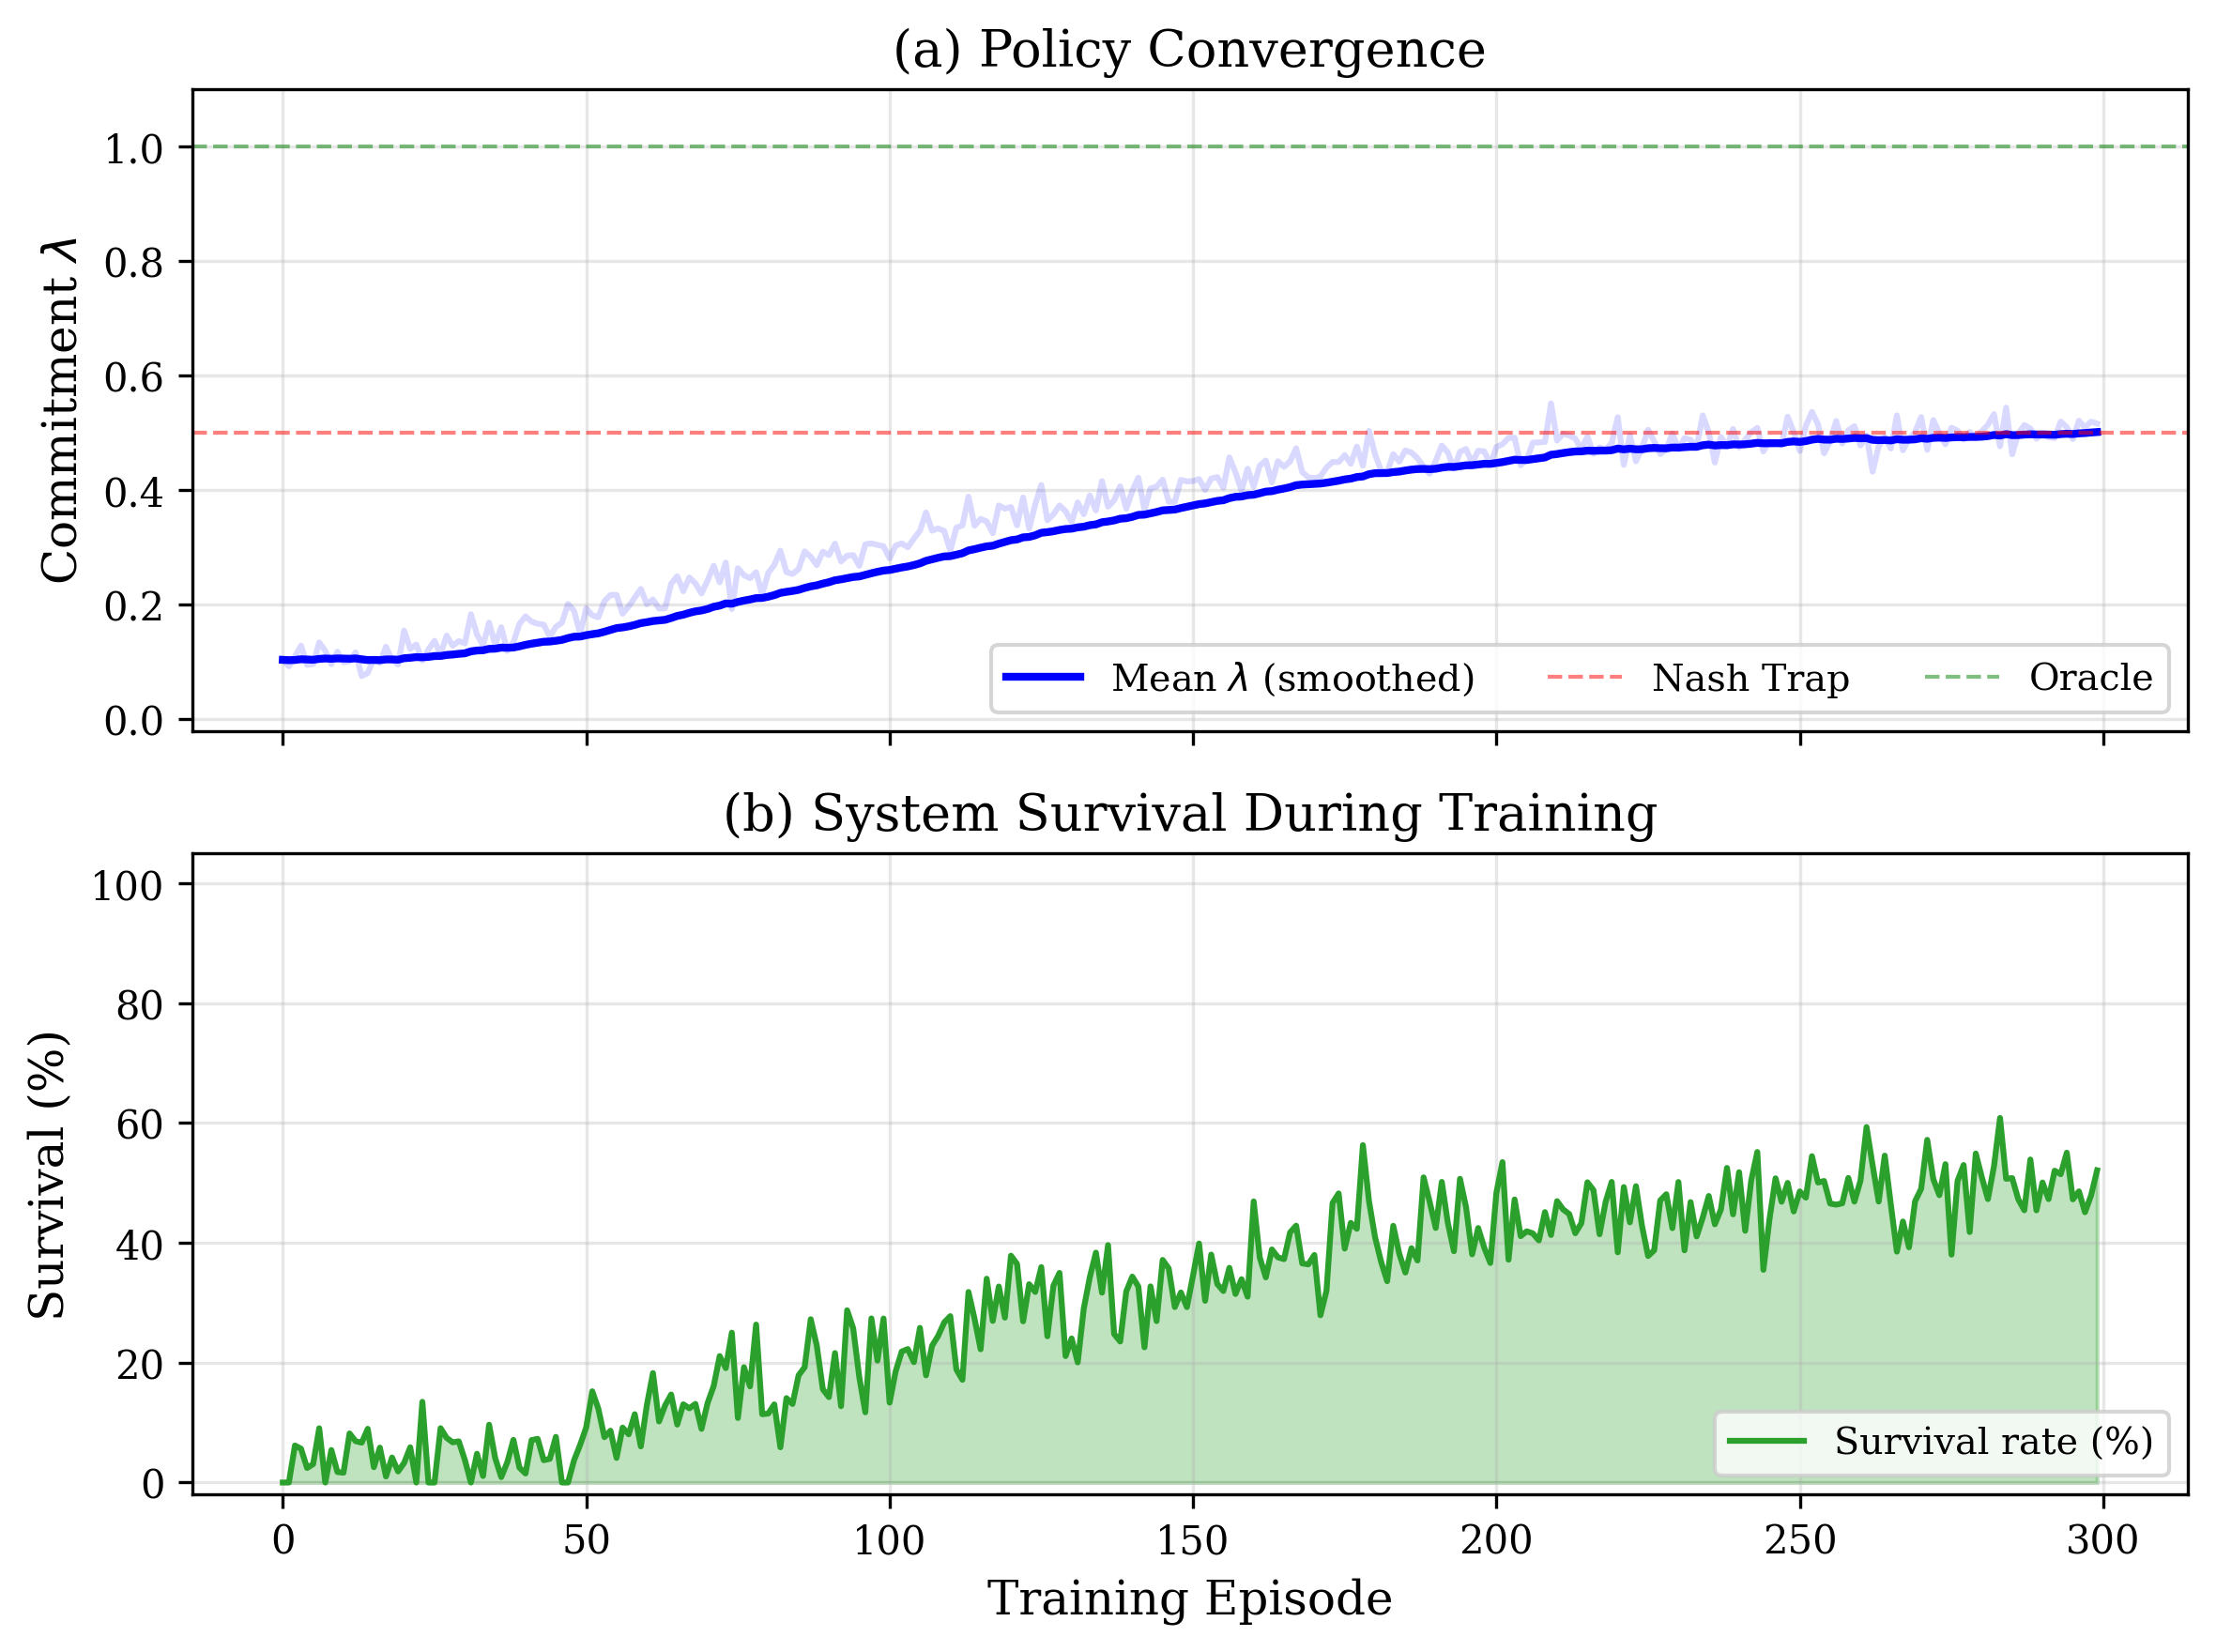
\includegraphics[width=\textwidth]{fig_p2_training_curves.png}
    \caption{RL training curves over 300 episodes (5 seeds, mean $\pm$ std). Left: clean environment; Right: 30\% Byzantine. Blue line: mean $\lambda$; red dashed: crisis $\lambda$ ($R_t < R_{\mathrm{crit}}$). Neither deviates from 0.5, confirming the Nash Trap. Green shading: system survival rate.}
    \label{fig:training_curves}
\end{figure}

\subsection{Result 2: Optimal Ethical Prior via Parameter Search}
\label{sec:hpo}

We optimize $g_\phi$ using finite-difference gradient estimation over the group welfare objective, sweeping $\phi_1$ (crisis commitment) across $[0, 1]$.

\begin{table}[t]
\centering
\caption{Effect of crisis commitment level $\phi_1$ on welfare and survival under stochastic shocks (SHOCK model, 20 seeds).}
\label{tab:phi1_sweep}
\begin{tabular}{ccccc}
\toprule
$\boldsymbol{\phi_1}$ & \textbf{W (Byz=0\%)} & \textbf{W (Byz=30\%)} & \textbf{Alive (Byz=0\%)} & \textbf{Alive (Byz=30\%)} \\
\midrule
0.00 & 27.2 & 22.6 & 60\% & 25\% \\
0.21 & 29.2 & 24.0 & 70\% & 35\% \\
0.50 & 30.8 & 25.7 & 85\% & 50\% \\
\textbf{1.00} & \textbf{32.0} & \textbf{28.2} & \textbf{100\%} & \textbf{90\%} \\
\bottomrule
\end{tabular}
\end{table}

Table~\ref{tab:phi1_sweep} shows that $\phi_1^* = 1.0$ is optimal across \emph{all} conditions.
This result is counter-intuitive: one might expect crisis commitment to decrease for self-preservation.
Instead, maximal commitment during crises accelerates resource recovery, preventing the system from crossing the tipping point.

\subsection{Result 3: Robustness of Unconditional Commitment}
\label{sec:robustness}

\paragraph{Individual Welfare.}
Under $\phi_1 = 1.0$, the bottom-10\% of agents (by cumulative payoff) earn \emph{more} than under $\phi_1 = 0.21$ (+587 at Byz=0\%, +250 at Byz=50\%), with Gini coefficients unchanged or reduced.
Unconditional commitment is Pareto-improving: no agent is worse off.

\paragraph{Adaptive Adversaries.}
We test an ``Exploitative Scarcity'' attack where adversaries strategically drain resources to exploit committed agents.
Result: welfare drops by $<$1.3\% under $\phi_1 = 1.0$, comparable to the 1.3\% drop under $\phi_1 = 0.21$.
The ``always-commit'' strategy does not create exploitable vulnerabilities.

% ================================================================
\section{Discussion}
\label{sec:discussion}

\subsection{Why RL Fails: The Structure of the Nash Trap}

The gradient vanishing at $\lambda = 0.5$ is not an artifact of policy network capacity.
It reflects a fundamental property of the PGG social dilemma: the marginal individual cost of increasing $\lambda$ (reduced retained endowment) is \emph{certain and immediate}, while the marginal collective benefit (resource preservation) is \emph{diffuse and delayed}.
Standard RL with discount factor $\gamma$ cannot bridge this gap because the Critic must learn to value a \emph{collective trajectory} (system survival over many rounds) from \emph{individual returns}---a credit assignment problem that compounds with the number of agents.

\subsection{Ethical Priors as Design Constraints}

Our findings suggest a design principle for autonomous multi-agent systems deployed in non-linear environments: \textbf{cooperative behavior must be architecturally guaranteed, not emergently hoped for}.
The commitment function $g(\theta, R)$ serves as a ``moral constitution''---a hard constraint that prevents the system from entering the Nash Trap, analogously to how safety constraints in control theory prevent physical systems from entering dangerous states~\cite{amodei2016concrete}.

\subsection{Connection to Sen's Theory of Commitment}

Amartya Sen~\cite{sen1977rational} argued that human behavior cannot be reduced to preference maximization; genuine ``commitment'' involves acting against one's immediate self-interest.
Our computational results provide unexpected support: the optimal $\phi_1^* = 1.0$ corresponds exactly to Sen's concept of \emph{unconditional} commitment---maintaining prosocial behavior regardless of personal cost.
That this emerges as mathematically optimal (not merely philosophically desirable) under non-linear dynamics is, to our knowledge, a novel finding.

\subsection{Limitations}

\begin{itemize}
    \item \textbf{Policy Complexity}: Our RL experiments use a linear policy ($\sigma(W^\top s + b)$).
    Deeper networks (MLP, attention) might discover more sophisticated strategies.
    However, the Nash Trap is a \emph{game-theoretic} property, not a function approximation limitation: even with perfect value estimation, the selfish optimum in PGG with $M/N < 1$ remains suboptimal.
    \item \textbf{Environment Scope}: Results are demonstrated in PGG with stylized non-linear dynamics.
    Validation in spatially-extended environments (e.g., SMAC, Melting Pot) is needed.
    \item \textbf{Parameter Search vs.\ Learning}: The ethical prior $g_\phi$ is optimized via grid search, not learned end-to-end.
    Meta-learning approaches (MAML) for $g$ remain future work.
\end{itemize}

% ================================================================
\section{Conclusion}

We have shown that purely selfish multi-agent reinforcement learning fails to discover cooperative strategies in environments with non-linear tipping points.
Agents converge to a Nash Trap ($\lambda \approx 0.5$) that is catastrophically insufficient under adversarial or stochastic conditions (5.3\% survival with 30\% Byzantine agents).
In contrast, agents equipped with a pre-specified ethical prior---a commitment function encoding Amartya Sen's concept of unconditional commitment---achieve 100\% survival and Pareto-improving welfare distribution.

These results carry a clear engineering implication: \textbf{autonomous multi-agent systems deployed in critical non-linear environments must incorporate ethical priors as hard design constraints, not optional features.}
Cooperation cannot be left to emerge from self-interest alone.

\section*{Broader Impact}

This work addresses the safety of multi-agent AI systems deployed in critical infrastructure (climate, finance, ecosystems).
Our finding that ethical priors are \emph{necessary}---not merely helpful---has direct implications for AI governance:
\begin{itemize}
    \item \textbf{Positive}: Provides rigorous justification for embedding cooperative constraints into autonomous systems before deployment, reducing catastrophic failure risks.
    \item \textbf{Caution}: The specific form of the ethical prior $g(\theta, R)$ encodes particular value judgments. Determining \emph{whose} values to encode requires interdisciplinary collaboration with ethicists, policymakers, and affected communities.
\end{itemize}

\bibliography{paper2_references}
\bibliographystyle{plain}

\end{document}
